% !TeX root = ../Book3.tex
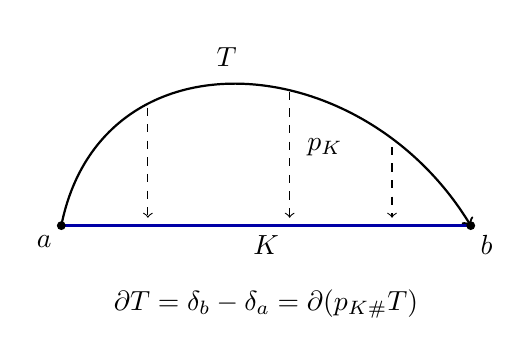
\begin{tikzpicture}[x=1cm,y=1cm]
	\draw[very thick,blue!65!black] (-2.6,0)--(2.6,0);
	\node[below] at (0,0) {\(K\)};
	\draw[thick,->] (-2.6,0) .. controls (-2.1,2.5) and (1.2,2.3) .. (2.6,0);
	\node[above] at (-0.5,1.9) {\(T\)};
	\draw[dashed,->] (-1.5,1.5)--(-1.5,0.1);
	\draw[dashed,->] (0.3,1.7)--(0.3,0.1);
	\draw[dashed,->] (1.6,1)--(1.6,0.1);
	\node[right] at (0.4,1) {\(p_K\)};
	\fill (-2.6,0) circle (1.6pt) node[below left] {\(a\)};
	\fill (2.6,0) circle (1.6pt) node[below right] {\(b\)};
	\node at (0,-1) {\(\partial T=\delta_b-\delta_a=\partial(p_{K\#}T)\)};
\end{tikzpicture}
